% !TEX program = pdflatex
\documentclass[a4paper,11pt]{article}
\usepackage[a4paper]{geometry}
%
%
\usepackage{graphicx}
\usepackage{amssymb,amsmath, amsthm}
\usepackage{mathrsfs}
\usepackage{bbm,bbold}
\usepackage{todonotes}
\usepackage{lineno}
\usepackage{enumitem}
\usepackage{booktabs}
\usepackage{caption}
\usepackage{subcaption}
\usepackage{wrapfig}

\usepackage{comment}

%%%%% THEOREM ENVIRONMENTS
\theoremstyle{plain}
\newtheorem{theorem}{Theorem}
\newtheorem{proposition}[theorem]{Proposition}
\newtheorem{lemma}[theorem]{Lemma}
\newtheorem*{lemma*}{Auxiliary Lemma}
\newtheorem{observation}[theorem]{Observation}
\newtheorem{corollary}[theorem]{Corollary}
\newtheorem{fact}[theorem]{Fact}
\newtheorem{conjecture}{Conjecture}
\newtheorem{problem}[theorem]{Problem}
\newtheorem*{conj1}{Conjecture 1}
\newtheorem*{conj2}{Conjecture 2}
\newtheorem*{conj1k2k}{Conjecture 1'}%$_{(k\hookrightarrow 2k)}$}

\theoremstyle{definition}
\newtheorem{definition}[theorem]{Definition}
\newtheorem{remark}[theorem]{Remark}
\newtheorem{remarks}[theorem]{Remarks}
\newtheorem*{acknowledgements}{Acknowledgements}
\newtheorem{example}[theorem]{Example}

\theoremstyle{remark}
\newtheorem{claim}{Claim}

%%% BOLD MATH
\newcommand{\myboldmath}[1]{\mathbbm{#1}}
\newcommand{\R}{\myboldmath{R}}
\newcommand{\G}{\myboldmath{G}}
\newcommand{\Q}{\myboldmath{Q}}
\newcommand{\N}{\myboldmath{N}}
\newcommand{\Z}{\myboldmath{Z}}
\newcommand{\F}{\myboldmath{F}}
\newcommand{\s}{\myboldmath{S}}
\newcommand{\C}{\myboldmath{C}}

\newcommand{\1}{\mathbf{1}}
\newcommand{\E}{\myboldmath{E}}

%%% SIMPLICIAL COMPLEXES AND GRAPHS
\DeclareMathOperator{\st}{st}
\DeclareMathOperator{\lk}{lk}
\newcommand{\bd}{\partial}
\newcommand{\im}{\operatorname{im}}

%%%% OTHER STUFF
\DeclareMathOperator{\supp}{supp}
\newcommand{\up}{\textup{up}}
\newcommand{\down}{\textup{down}} 


\begin{document}
\linenumbers

%%%%OPENING
\title{Hit and Run and Stuff}
\author{Brian Cohn \and May Szedl\'{a}k \and Francisco Valero-Cuevas \and Bernd G{\"a}rtner \and Komei Fukuda}
\begin{titlepage}
\maketitle
\thispagestyle{empty}
%%
The families of solutions for a particular motor task  (i.e., feasible activation sets) are high-dimensional subspaces with a well defined structure that emerges naturally from the interactions among the feasible neural commands, the anatomy of the limb, and the mechanical constraints defining the task.
Characterizing their structure, however, has proven challenging.
Here we present a novel computationally efficient approach to characterize their multi-dimensional structure by uniformly sampling their interior using the Hit-and-Run algorithm---a generalization of a discrete Markov chain.
We studied 3D static force production by a realistic model of the human index finger with 7 muscles and 4 kinematic degrees of freedom.
For each of 9 sub-maximal magnitudes of static fingertip force in a given direction, the feasible activation set is a 4-dimensional convex polytope  embedded in 7-dimensional activation space.
We describe the structure of each feasible activation set by the histograms of feasible activations for individual muscles.  Then, we describe the multi-dimensional interaction among these valid muscle activations and six cost functions using an interactive parallel coordinates system. 
This first description of the multi-dimensional nature of families of feasible solutions  has important consequences to our understanding of the neural control of redundant musculature.  For example, the bounding box of the feasible activation set singularly misconstrues the families of feasible activations—and the modes of the histograms for low magnitudes do not necessarily correspond to those for higher ones. Similarly, exploring and exploiting families of feasible solutions is likely more biologically plausible than searching for unique optimal solutions, and knowing these families will help mitigate biomechanical confounds in dimensionality reduction techniques seeking to extract synergies of neural origin.
More importantly, describing the structure of feasible activation sets as raw or cost-weighted multi-dimensional probability distributions marries neuromechanical and Bayesian perspectives into an integrative probabilistic approach to motor control, dysfunction, rehabilitation, and learning/adaptation for neuromechanically realistic limbs.
%%
\end{titlepage}
%%%%

%%%%ARTICLE
\section{Author Summary}
brian is a phd student\\
may is a phd student\\
bernt, komei, and francisco are professors
\section{Introduction}

Optimal control of a musculoskeletal system is intrinsically related to mechanical constraints. 
An endpoint's end effector forces are highly dependent upon tendon force ranges, the leverage of each tendon insertion point across each joint, and the planes of motion each degree of freedom (DOF), with these physical relationships defining the capabilities of the system.
In spite of the complexity of alpha-gamma neuromuscular drive models, every system exists under limitations intrinsic to physical mechanics, and as such, limbs have been modeled to behave under these constraints with stunning realism [cite]. With increasingly accurate and faceted models, a great body of research has been tasked with predicting kinetics, while being sensitive to subtle changes in muscle activation [todorov's mujoco], skeletal weight distributions, neural synergies, and spatiotemporal variables[Kornelius and FVC, Racz FVC].
While many of these models highlight their accuracy , and attribute it to nonlinear dynamic modeling, linear approximation has long-remained a viable way to interpret the actions of physical limb systems, in the context of a well-understood mathematical framework.
As limbs exist under physical constraints, neuromuscular control must strategize within the generic Newtonian laws of physics, in the realm of linear statics and dynamics.
While some would argue that linear approximation of a musculoskeletal system is a blunt instrument in researching what is considered a 'non-linear' system, linear approximation can offer a 'big picture view' of the system.
Some attention has been given to the constraints that physical systems impart on control itself ['nice try' citations], with many placing emphasis on non-linear synergies between motor units, for instance, between the \textit{vastus lateralis} and \textit{vastus medialis} muscles of the leg.
A breadth of modeling techniques have been applied to physical systems to model and understand CNS control under the constaints of a given task, and many have been able to visualize some of the limitations animals must abide by in optimization.

Optimal control theory must be implemented in a way such that it is computationally tractable. Control systems of designed (robotic) and evolved (neurophysiologic) origins can afford only a small measure of latency.
Identifying how optimal control works within the framework of constraints could bring rise to more efficient algorithms, and this contextual understanding could introduce new ways to visualize how neuromuscular systems learn to improve over training.
In dynamic systems we have seen <do research on this>[cite].

In a static system, every possible combination of independent muscle activations exists within the unit-n-cube, where N is set to however many independently-controlled muscles a system has.
Prior work has highlighted the relationship between the feasible force space and the set of all activation solutions.[cite papers in the last 10 years]
In effect, adding constraints on the FFS (e.g. requiring only force in a given plane) adds constraints to the FAS

The effect of each muscle on each joint has been represented by the moment arm matrix [citations], the relationship of each DOF on end-effector output directions .
The feasible force set (described in detail in [cite]) is an M-dimensional polytope containing all possible force vectors an endpoint can output.

neurons do alot of stuff, and much work has been put into understanding how neural drive results in force, motion, and kinetics. 
physical description of a musculoskeletal system


Functional performance is defined by the ability for a system to identify optimal solutions in a set of suboptimal solutions. 
<talk about local and global maxima and minima in neuro optimization control theory>

The feasible force set represents every possible output force an end effector can impart on an endpoint.






Described in a mathematical way the feasible activation set is expressed as follows. For a given force vector $f \in \mathbb{R}^m$, which are the activations that satisfy
\[\textbf{f} = A\textbf{a}, \textbf{a} \in [0,1]^n?\]
In our 7-dimensional example $m =4$ and $n =7$, typically $n$ is much larger than $m$.
The constraint $\textbf{a} \in [0,1]^n$ describes that the feasible activation space lies in the $n$-dimensional unit cube (also called the $n$-cube). Each row of the constraint $\textbf{f} = A\textbf{a}$ is a $n-1$ dimensional hyperplane. Assuming that the rows in $A$ are linearly independent (which is a safe assumption in the muscle system case), the intersection of all $m$ equality constraints constraints is a $(n-m)$-dimensional hyperplane. Hence the feasible activation set is the polytope given by the intersection of the $n$-cube and an $(n-m)$-dimensional hyperplane. Note that this intersection is empty in the case where the force $f$ can not be generated.


Issues with volume computations:
As realistic musculoskeletal systems has many more muscles, it's important for polytope calculation to be scalable to higher dimensions.


We first describe the stochastic method of hit-and-run, and illustrate its use on a fabricated 3-muscle, 1-DOF system with a desired force output of 1N. We designed this schematic (but mathematically viable) linear system of constraints to help readers understand the mechanics of hit-and-run mathematics. Our index-finger model has too many dimensions to show how the process works, so we hope this will help readers understand what is going on in n dimensions (7 in the case of the index-finger model). We also used this model to perform unit tests on our code in thoroughly validating our hit-and-run implementation.

We investigated the distributions of the feasible activation set across each muscle.
State the purpose of the work in the form of the hypothesis, question, or problem you investigated; and,
Briefly explain your rationale and approach and, whenever possible, the possible outcomes your study can reveal.

\section{Materials and Methods}

% TODO Insert the J and R matrices, and show their multiplication
% Sample Calculation X.

% TODO Insert the F_o Vector
% Table X.


% TODO Insert the A matrix, ith full muscle names
% Table X. Each column represents a wrench generators (with each dimension in Newtons). The muscle is modeled such that full activation would produce the column of forces and torque at the fingertip.


\subsection{Data and Samples}
We began with an index finger of a healthy human (male) right hand, which was taken from []. The hand size, finger lengths, and weight was []. Dissected by []. Experimental forces from [].
All procedures were performed under protocol of the [] university standards, and the study was approved by []. 
The moment arm matrix, $R$, which contains the leverage of each tendon's insertion points across each joint, was measured by doing [], [] ,and then [].
The Jacobian, $J$, which represents the effect of rotation at each DOF on each component of endpoint wrench [cite jacobian usage], was measured with a [], by [], with precision of $\pm x$.
The force-naught vector, $F_0$, which contains the tendon force at maximal isometric contration (MIC)[cite method used] for each muscle, was taken in the [same or different] posture, with a [] measuring device, with precision of $\pm x$.



\subsection{Polytope representation of the feasible activation space}
Exact volume calculations for polygons can only be done in reasonable time in up to 10 dimensions \cite{Dyer2, Khachiyan, Khachiyan2}. We therefore use the so called Hit-and-Run approach, which samples a series of points in a given polygon. Given the points for a feasibale activation space, this method gives us a deeper understanding of its underlying structure. 



\subsection{Hit-and-Run}
In this section we introduce the Hit-and-Run algorithm used for uniform sampling in a convex body $K$, was introduced by Smith in 1984 \cite{Smith}. The mixing time is known to be $\mathcal{O}^*(n^2R^2/r^2)$, where $R$ and $r$ are the radii of the inscribed and cicumscribed ball of $K$ respectively \cite{Dyer, Lovasz}. I.e., after $\mathcal{O}^*(n^2R^2/r^2)$ steps of the Hit-and-Run algorithm we are at a uniformly at random point in the convex body. 
In the case of the muscles of a limb, we are interested in the polygon $P$ that is given by the set of all possible activations $\textbf{a} \in \mathbb{R}^n$ that satisfy
\[\textbf{f} = A\textbf{a}, \textbf{a} \in [0,1]^n,\]
where $\textbf{f} \in \mathbb{R}^m$ is a fixed force vector and $A = J^{-T}RF_m \in \mathbb{R}^{m \times n}$. $P$ is bounded by the unit $n$-cube since all variables $a_i$, $i \in [n]$ are bounded by 0 and 1 from below, above respectively.
Consider the following $1 \times 3$ fabricated example.
\begin{align*}
&1 = \frac{10}{3}a_1 - \frac{53}{15}a_2 + 2a_3 \\
&a_1, a_2, a_3 \in [0,1],
\end{align*}
the set of feasible activations is given by the shaded set in Figure \ref{fig_hr}.

\begin{figure}[ht]
   \begin{center}
    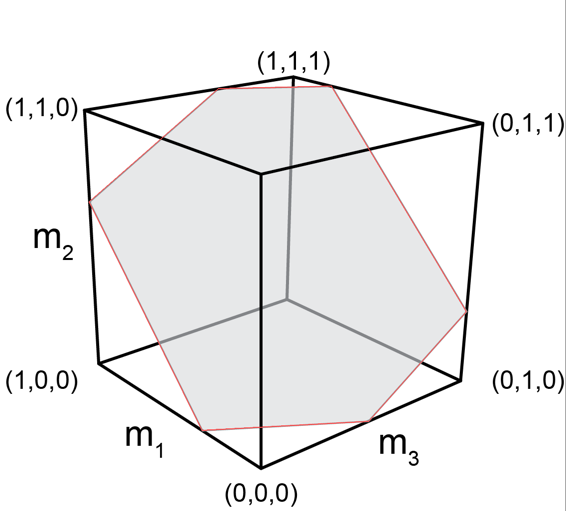
\includegraphics[width=0.25\textwidth]{feasibleactivation.png}
  \end{center}
  \caption{Feasible Activation}
  \label{fig_hr}
\end{figure}

The Hit-and-Run walk on $P$ is defined as follows (it works analogously for any convex body). 
\begin{enumerate}
\item Find a given starting point $\textbf{p}$ of $P$ (Figure \ref{fig_hr1}) .
\item Generate a random direction through $\textbf{p}$ (uniformly at random over all directions) (Figure \ref{fig_hr2}).
\item Find the intersection points of the random direction with the $n$-unit cube (Figure \ref{fig_hr3}).
\item Choose the next point of the sampling algorithm uniformly at random from the segment of the line in $P$ (Figure \ref{fig_hr4}). 
\item Repeat from $(b)$ the above steps with the new point as the starting point .
\end{enumerate}


\begin{figure}
        \centering
        \begin{subfigure}[b]{0.25\textwidth}
                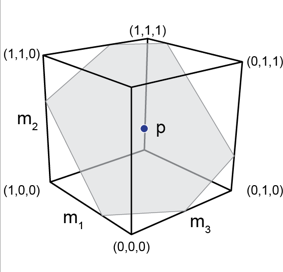
\includegraphics[width=\textwidth]{HR2.png}
                 \caption{Inner Point}
      						\label{fig_hr1}
        \end{subfigure} \hspace{0.5cm}
        \begin{subfigure}[b]{0.25\textwidth}
                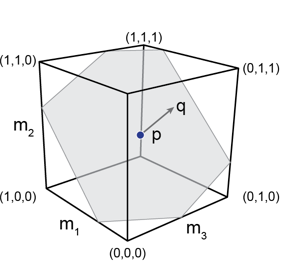
\includegraphics[width=\textwidth]{HR3.png}
                \caption{Direction}
      					\label{fig_hr2}
        \end{subfigure} \\
        \begin{subfigure}[b]{0.25\textwidth}
                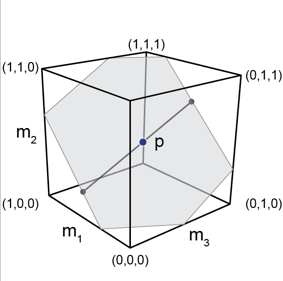
\includegraphics[width=\textwidth]{HR4.png}
                 \caption{Endpoints}
      					\label{fig_hr3}
        \end{subfigure} \hspace{0.5cm}
        \begin{subfigure}[b]{0.25\textwidth}
                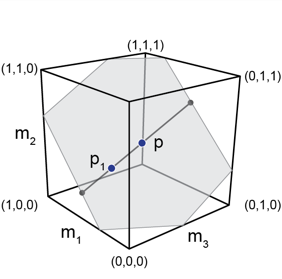
\includegraphics[width=\textwidth]{HR5.png}
                \caption{New Point}
      				 \label{fig_hr4}
        \end{subfigure}
        \caption{Hit-and-Run Step}\label{fig:animals}
\end{figure}

%\begin{figure}[ht]
%   \begin{center}
%    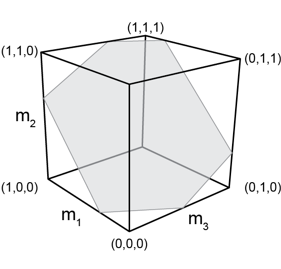
\includegraphics[width=0.25\textwidth]{HR1.png}
%      \caption{Inner Point}
%      \label{fig_hr1}
%    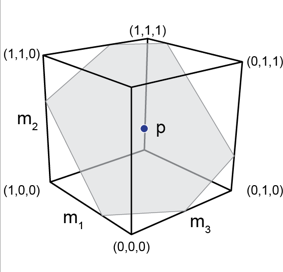
\includegraphics[width=0.25\textwidth]{HR2.png}
%    \caption{Direction}
%      \label{fig_hr2}
%    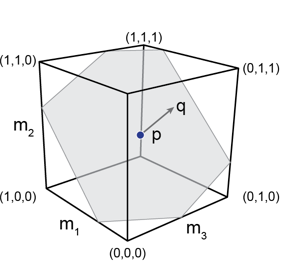
\includegraphics[width=0.25\textwidth]{HR3.png}
%    \caption{Endpoints}
%      \label{fig_hr3}
%    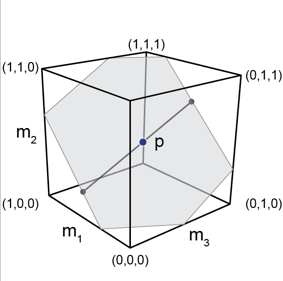
\includegraphics[width=0.25\textwidth]{HR4.png}
%    \caption{New Point}
%      \label{fig_hr4}
%  \end{center}
%\end{figure}

\begin{figure}[ht]
   \begin{center}
    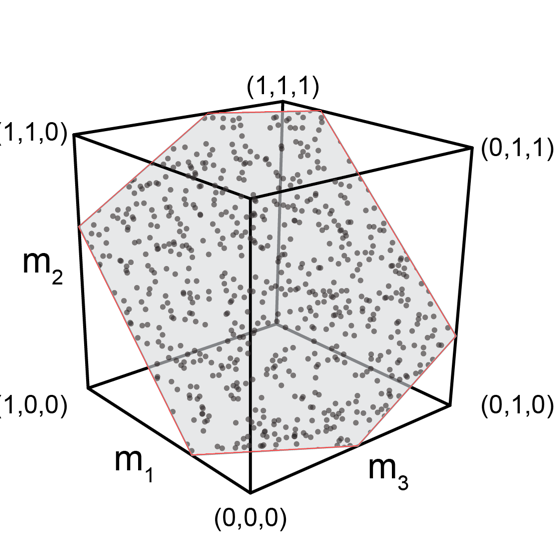
\includegraphics[width=0.25\textwidth]{uniform.png}
      \caption{Uniform Distribution}
      \label{fig_hr5}
  \end{center}
\end{figure}


The implementation of this algorithm is straight forward except for the choice of the random direction. How do we sample uniformly at random (u.a.r.) from all directions in $P$? Suppose that $\textbf{q}$ is a direction in $P$ and $p \in P$. Then by definition of $P$, $\textbf{q}$ must satisfy $\textbf{f} = A(\textbf{p}+\textbf{q})$. Since $\textbf{p} \in P$, we know that $\textbf{f} = A\textbf{p}$ and therefore 
\[\textbf{f} = A(\textbf{p} + \textbf{q}) = \textbf{f} + A\textbf{q}\]
and hence
\[A\textbf{q} = 0.\]

We therefore need to choose directions uniformly at random from all directions in the vectorspace 
\[V = \{\textbf{q} \in \mathbb{R}^n | A\textbf{q} = 0\}.\]

As shown by Marsaglia this can be done as follows \cite{Marsaglia}.

\begin{enumerate}
\item
Find an orthonormal basis $b_1, \dots, b_r \in \mathbb{R}^{n}$ of $A\textbf{q} =0$.
\item
Choose $(\lambda_1, \dots, \lambda_r) \in \mathcal{N}(0,1)^n$ (from the Gaussian distribution).
\item
$\sum_{i=1}^r \lambda_i b_i$ is a u.a.r.\ direction.
\end{enumerate}

A basis of a vectorspace $V$ is a minimal set of vectors that generate $V$, and it is orthonormal if the vectors are pairwise orthogonal (perpendicular) and have unit length. Using basic linear algebra one can find a basis for $V = \{A\textbf{q} = 0\}$ and orthogonalize it with the well known Gram-Schmidt method (for details see e.g.\ \cite{Robertson}). Note that in order to get the desired u.a.r.\ sample the basis needs to be orthonormal. For the limb case we can safely assume that the rows of $A$ are linearly independent and hence the number of basis vectors is $n-m$.



\begin{figure}
        \centering
        \begin{subfigure}[b]{0.25\textwidth}
                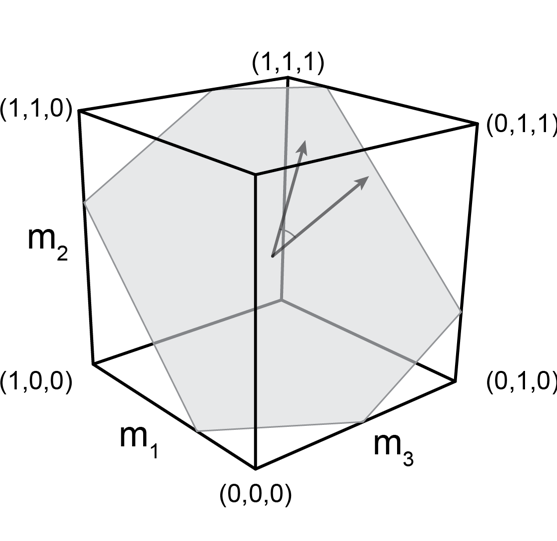
\includegraphics[width=\textwidth]{somebasis.png}
      \caption{Some Basis}
      \label{fig_somebasis}
              \end{subfigure} \hspace{0.5cm}
        \begin{subfigure}[b]{0.25\textwidth}
                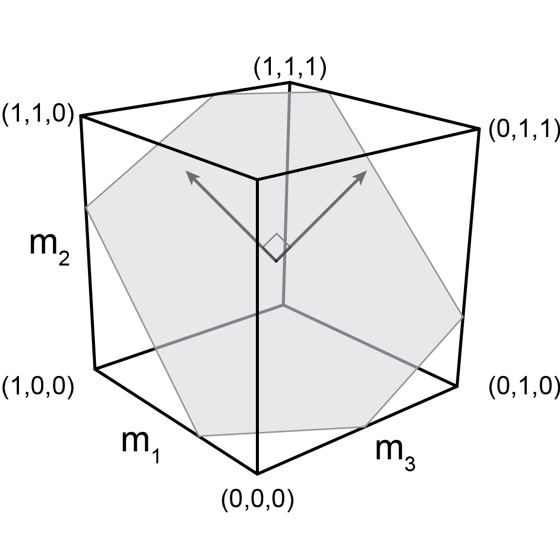
\includegraphics[width=\textwidth]{orthobasis.png}
     \caption{Direction}
      \label{Orthonormal Basis}        
      \end{subfigure}
      \caption{Find Orthonormal Basis}\label{fig_basis} 
\end{figure}


\subsection{Mixing Time}
How many steps are necessary to reach a uniformly at random point in the polytope? The theoretical bound $\mathcal{O}^*(n^2R^2/r^2)$ given in \cite{Lovasz} has a very large hidden coefficient ($10^30$) which makes the algorithm almost infeasible in lower dimensions.

These bounds hold for general convex sets. For convex polygons in higher dimensions, experimental results suggest that $\mathcal{O}(n)$ steps of the Hit-and-Run algorithm are sufficient. In particular Emiris and Fisikopoulos paper suggest that $(10 + 10\frac{n})n$ steps are enough to have a close to uniform distribution \cite{Emiris}. In all cases tested, sampling more point did not make accuarcy significantly higher. 

Ge et al.\ showed experimentally that up to about 40 dimensions, ??? random points seem to suffice to get a close to uniform discussion \cite{Ge}. 

Therfore for given output force we execute the Hit-and-Run algorithm 1000 times on 100 points. The experimental results propose that those 1000 points are uniformly distributed on the polygon.

As a additional control, for each muscle we observe that the theoretical upper and lower bound of the feasible activation match the observed corresponding bounds (difference max ??). To find the theoretical upperbound (lowerbound) of a given muscle activation we solve two linear programs maximizing (minimizing)  $a_i$ over the polytope.


%For the upper and lower bounds of the activation we can solve two linear program for each coordinate of $\textbf{a}$ to find the upper and lower bounds of each $a_i$.
%We see that those theoretical bounds match the experimentally obtained bounds.

\subsection{Starting Point}
To find a starting point in 
\[\textbf{f} = A\textbf{a}, \textbf{a} \in [0,1]^n,\]
we only need to find a feasible activation vector. For the hit and run algorithm to mix faster, we do not want the starting point to be in a vertex of the activation space. We use the following standard trick using slack variables $\epsilon_i$.

\begin{equation}\label{eq:LP_r}
\begin{array}{lrcl}
\mbox{maximize} & \sum_{i=1}^n \epsilon_i \\ 
\mbox{subject to} & \textbf{f} &=& A\textbf{a}\\
  & a_i &\in& [\epsilon_i, 1- \epsilon_i], \hspace{5mm} \forall i \in \{1,\dots,n\}  \\
  & \epsilon_i &\geq& 0, \hspace{5mm} \forall i \in \{1,\dots,n\}.  
\end{array}
\end{equation}

This approach can still fail in theory, but this method has the choose $\epsilon_i > 0$ and therefore $a_i \neq 0$ or $1$. Since for all vertices of the feasible activation space lie on the boundary of the $n$-cube, at least $n-m$ muscles must have activation $0$ or $1$. Documentation is included in our supplementary information.

\subsection{Parallel Coordinates: Visualization of the Feasible Activation Space}
Citation
A common way to visualize higher dimensional data is using parallel coordinates. To show our sample set of points in the feasible activation space we draw $n$ parallel lines, which representing the activations of the $n$ muscles. Each point is then represented by connecting their coordinates by $n-1$ lines.


\begin{figure}[ht]
   \begin{center}
    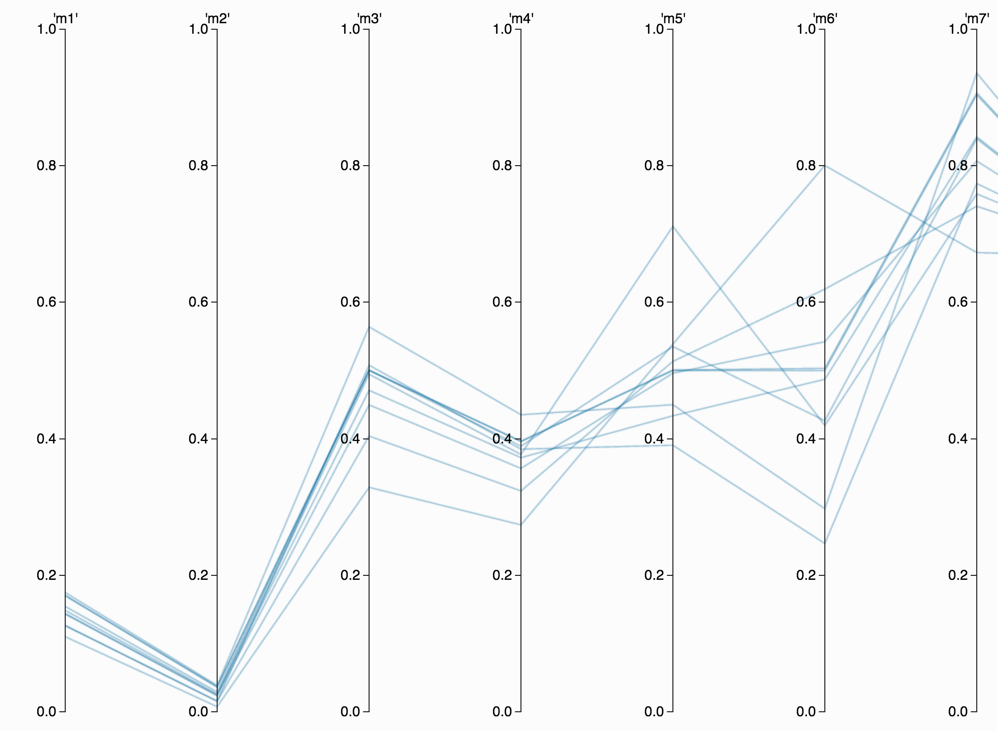
\includegraphics[width=0.5\textwidth]{pc.png}
  \end{center}
  \caption{Feasible Activation}
  \label{fig_pc}
\end{figure}

Using an interactive surface one can now restrict each muscle function to any desired interval, e.g., figure ??.

\textbf{NICE FIGURE OF RESTRICTED PARALLEL COORDINATES}

For the $l_1$, $l_2$ and $l_3$ norm respectively, we added an additional line to represent the corresponding weight. E.g.\ for a given point $\textbf{a} \in \mathbb{R}^n$ we are interested in $\sum_{i=1}^n a_i$, $\sqrt{\sum_{i=1}^n a_i^2}$ and $\sqrt[3]{\sum_{i=1}^n a_i^3}$. As for the muscles one can restrict the intervals of the weight functions, to explore the corresponding feasible activation space. 

\textbf{NICE PICTURE WITH WEIGHTS INCLUDED}
\begin{figure}[htbp]
\centering
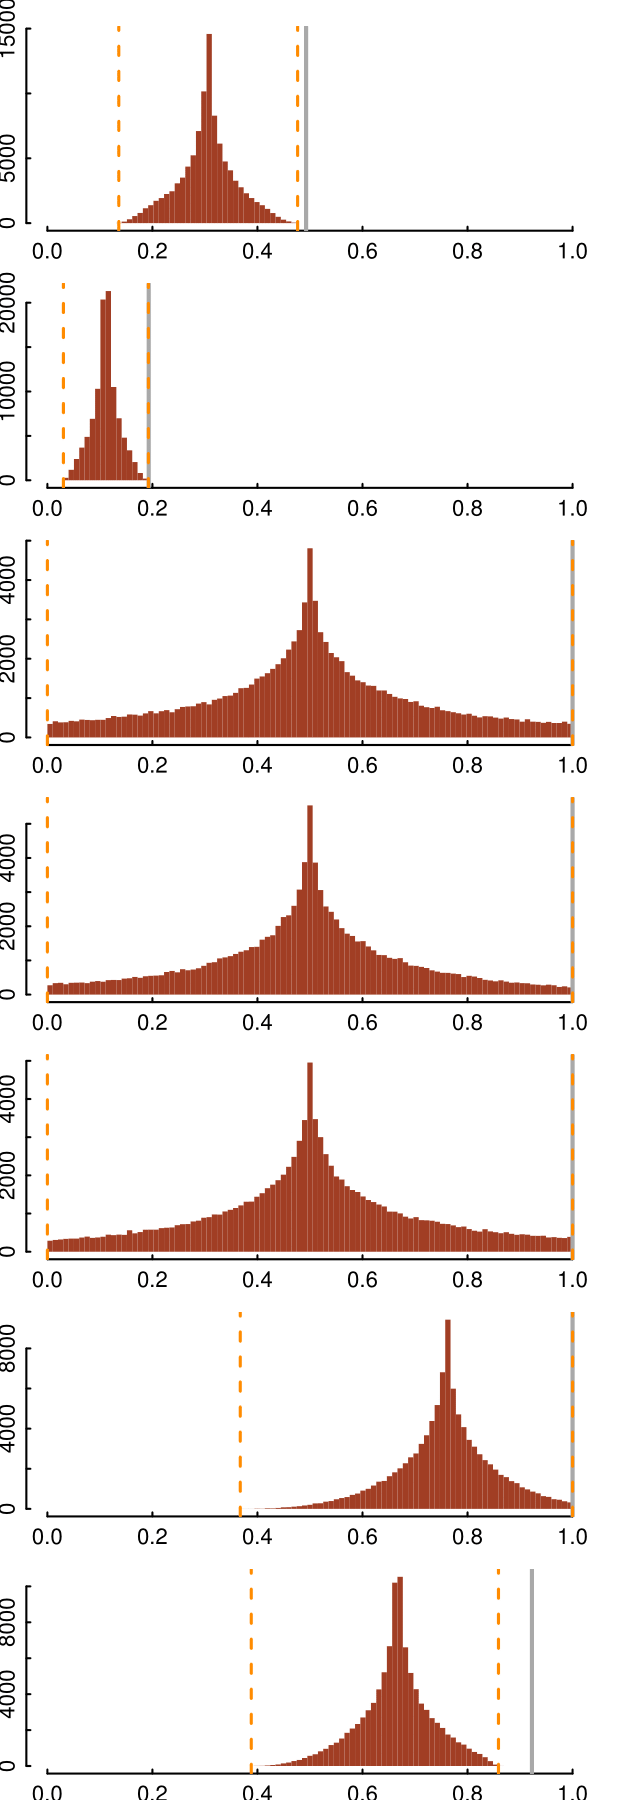
\includegraphics{sections/figs/raw_histograms.png}
\caption{Distribution of feasible activations for 50\% maximal force output in the palmar direction.}
\label{fig:raw_histograms}
\end{figure}


briantodo: add the following figures:
\begin{itemize}
\item{parcoord Full}
\item{parcoord muscle limited to 75\percent, then 50\percent, then 25\percent}
\item{}


\section{RESULTS}

Using Hit-and-Run to sample feasible activation sets, Figure \ref{fig:raw_histograms} shows the distributions of activation solutions for a palmar submaximal force.resulting from $1,000,000$ solutions computed with Hit-and-Run sampling. This is the first time (to our knowledge) that the internal structure of the feasible activation set has been visualized for a sub-maximal force.

Notice also that the lower and upper bounds of the activations (i.e., the dashed lines that indicate their bounding box), are uniquely uninformative of the actual density of distribution of feasible activations. Note also that the activation needed for the maximal force output (thick gray line) is very often not the mode of the activations at 50\% of output.


Results:
Projection onto a given muscle dimension
Simple histograms at 80% activation for one direction
Activation progression-march (3) x y z
Parallel coordinates with cost
	Full
Parallel Coordinates with cost
	Lower
	Middle
	Upper
	constraint by cost
		Yes you could put activation constraints directly in the A matrix, instead of bounds between 0 and 1. There is no advantage to adding activation constraints beforehand in the A matrix, as sampling is uniform- as long as the resulting dataset is large enough for your purpose.
		You could also put l1 and weighted l1 cost bounds as constraints in the A matrix. Cannot put higher order cost functions such as l2,l3 or weighted l2,l3.

		Talk about slopes in Parallel
		if they 


\section{DISCUSSION}

\subsection{Level of trust of the polytope approximation} % (fold)
\label{sub:level_of_trust_of_the_polytope_approximation}

Our approximations show sufficiently accurate views of the polytope in slices perpendicular to each axis. Had we performed exact volume computations, we would have had more accurate relative volumes; that said, the level of error generated through approximation is exceptionally small in comparison to error derived from measuring/predicting the musculoskeletal parameters to define the force generators $A$. Our code only solves one linear equation to find the starting point, and the time-cost of each point thereafter is linear; therefore this method can be used for tendon driven models in very high-dimensional systems.

Sohn et. al. have identified how the bounding box can illustrate the bounds of feasible activation; essentially reducing the effective number of solutions a neuromuscular system can select from \cite{sohn2013cat_bounding_box}. Our research here looks to further constrain this space by observing the cost-agnostic distribution of solutions across the set of all feasible coordination patterns.

% subsection level_of_trust_of_the_polytope_approximation (end)
\subsection{Activation Progression} % (fold)
\label{sub:activation_progression}
The only way that the bounding box would contain the entire set of information regarding a given muscle's activation distribution would be if that end effector is completely unaffected by any activation of that muscle i.e. the muscle's linear endpoint force is the 0 vector. As such, muscles which are nearly uninvolved in the end effector's actions will form near-uniform distributions, as their involvement does not affect the activation space.
% subsection activation_progression (end)

\subsection{Features of the PDF} % (fold)
\label{sub:features_of_the_pdf}
why must they be \\
unimodal\\
non-normal\\
non-uniform (talk about the exception(s))\\
what the exact pdf function would be \\
	a piecewise quadratic equation, where it changes when you incorporate/exclude vertices of the polytope
% subsection features_of_the_pdf (end)

\subsection{Parallel coordinate slopes} % (fold)
\label{sec:parallel_coordinate_slopes}
[maytodo: Talk about what it means to have slopes in Parallel, what a very positive slope means/what a very negative slope means, and what the crossing-slopes mean. Also put forward a couple suggestions of how these slopes could be more quantitatively interpreted/analyzed]
% subsection parallel_coordinate_slopes (end)

\subsection{Cost distributions} % (fold)
\label{sec:cost_distributions}
In further studies one could put activaton constraints directly into the $A$, instead of the unit interval bounds. As long as the resulting dataset is large enough for our purpose, there is no advantage to this, as we can not compare with the original feasible activation space. Since $l_1$ and $l_1^w$ are linear, one can also put corresponding constraints into $A$. Our implementation does not support directily inputting bounds on the higher degree weight functions $l_2$, $l_3$, $l_2^w$ and $l_3^w$.
%Yes in further studies we could put activation constraints directly in the A matrix, instead of bounds between 0 and 1. But there are no advantages to adding activation constraints beforehand in the A matrix, as sampling is uniform- as long as the resulting dataset is large enough for your purpose.
%You could also put l1 and weighted l1 cost bounds as constraints in the A matrix. Cannot put higher order cost functions such as l2,l3 or weighted l2,l3.

We note that the activation and metabolic classes of cost function are fundamentally different, and do not explore correlations between these two classes. We do, however, note that when all of the involved cost functions are 'minimized' to the bottom half of all solution costs, the union maintains a very high number of solutions (22\%). With this we can note how all of these cost functions are similar in nature across the polytope (as expected).
% subsection cost_distributions (end)

\subsection{Concluding remarks} % (fold)
\label{ssub:concluding_remarks}

Our results clearly show:
\begin{itemize}
	\item{The Hit-and-Run algorithm can explore the feasible activation space for a realistic 7-muscle finger in a way that is computationally tractable.}
	\item{We find that the bounding box exceptionally misconstrues the internal structure of the feasible activation set.}
	\item{The Hit-and-Run algorithm is cost-agnostic in the sense that no cost function is needed to predict the distribution of muscle activation patterns. Therefore, we can provide spatial context to where 'optimal' solutions lie within the solution space; this approach can be used to explore the consequences of different cost functions.}
	\item{The distribution of muscle activations often show and strong modes that will critically affect the learning of motor tasks.}
\end{itemize}
In comparison to traditional bounding-box representations, our application of Hit-and-Run in this context is decisively superior in capability for meaningful visualization, value in extracting associations between solutions, and computational tractability, in addition to being veritable of the true solution distributions within the feasible activation set. Our bodies exist within a feasible activation space, and once we enter this space then optimization is possible. In this way, we can think of the solutions space as an effectie model for exporation-exploitation.
This can help us in comparing the structure of the activation space as a set of high-dimensional bayesian priors which are narrowed/shifted over time to compensate for learning and skill-development.
Essentially, once you enter into task-independent variation, it becomes a question of identifying the region of the activaiton space which both satisfieds the spatiotemporal constraints, but also approaches optimality under efficiency/speed demands.
We want to 'close the loop' between the nervous system commands, and the mechanical output, thereby uncovering how the CNS collaborates with newtonian physics to select neural commands which effecitvey coordinate multi-link limbs, so we can act, play, and dance in the real world.
Mechanical demands constrain the total space of musculoskeletal coordination options, thus, motile organisms first 'explore' coordination strategies conducive to the desired movement, and recursively redefine the more optimal subspaces.
Once a desired task is mapped to an effective coordination strategy (as in, it gets the job done), then training and experience (exploration-exploitation) can aid in finding the best coordination.
As many tasks are similar (ie. they require the similar force generation or torque production over the course of a movement),  the activation patterns for simlar actions must be similar as well.
Optimal coordination strategies for one task may be near-optimal for a similar task.
On the other hand, a suboptimal coordination strategy that achieves one task, may be furiously off-target for a very similar task.

intention --> excitation --> activation dynamics --> contraction properties --> muscle properties with muscle models --> musculoskeletal force on the bones, joints, and finally, endpoint force. Long chain and we only look at 2 parts.

[briantodo: discuss francisco's paper about scaling the solution to the boundary.]

% subsubsection concluding_remarks (end)

[briantodo: address the following:]
any given manuscript must satisfy the following criteria:
\begin{itemize}
	\item {Originality}
	\item {Innovation}
	\item {High importance to researchers in the field}
	\item {Significant biological and/or methodological insight}
	\item {Rigorous methodology}
	\item {Substantial evidence for its conclusions}
\end{itemize}



We thank all of the people.


\bibliographystyle{plain}
\bibliography{redundancyFVC}
%\section{APPENDIX}

\subsection{Finger model data}
$F_o = (123.0, 219.0, 23.52, 91.74,	21.6, 124.8, 129.6)$\\
$
JR = 
\begin{pmatrix}
-0.08941 & -0.0447 & -0.009249 & 0.03669 & 0.1421 & 0.2087 & -0.2138 \\
-0.04689 & -0.1496 & 0.052 &0.052 & 0.0248 & 0.0 & 0.0248 \\ 
0.06472 & 0.001953 & -0.1518 &-0.1518 & 0.2919 & 0.0568 & 0.2067 \\
0.003081 & -0.002352 & -0.0001649 & -0.0001649 & -0.0004483 & 0.0001578 & -0.000685
\end{pmatrix}
$
$task_x = (1.0,0.0,0.0,0.0)$
$task_y = (0.0,1.0,0.0,0.0)$
Palmar force is $task_z = (0.0,0.0,1.0,0.0)$
$task_xy = (1.0,1.0,0.0,0.0)$

\begin{figure}[h]
\centering
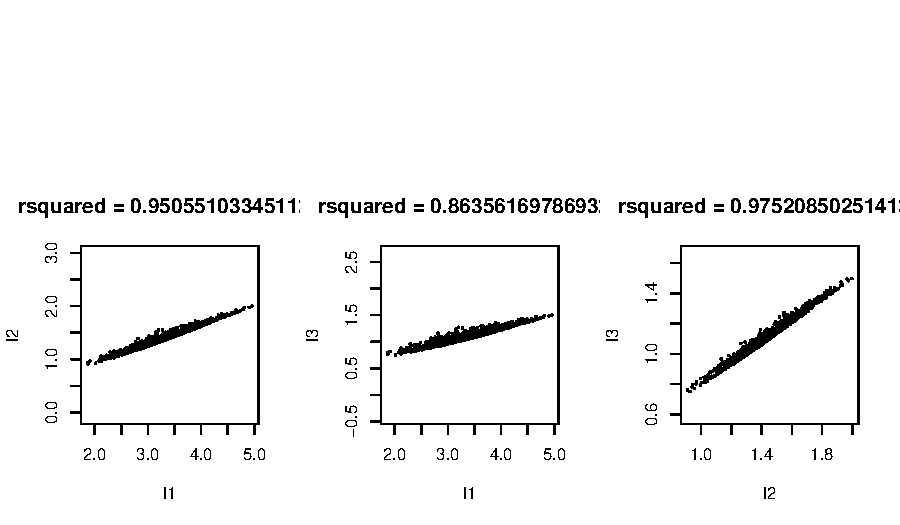
\includegraphics[width=0.5\textwidth,page=1]{figs/cost_function_scatterplots.pdf}
\caption{Nonweighted cost functions}
\label{fig:unweighted_cost_functions}
\end{figure}

\begin{figure}[h]
\centering
\includegraphics[width=0.5\textwidth,page=2]{figs/cost_function_scatterplots.pdf}
\caption{Weighted cost functions}
\label{fig:weighted_cost_functions}
\end{figure}
\end{document}
